\documentclass[12pt]{article}

\usepackage{amsmath}
\usepackage[margin = 1in]{geometry}
\usepackage{graphicx}
\usepackage{booktabs}
\usepackage{natbib}

% for space filling
\usepackage{lipsum}
% highlighting hyper links
\usepackage[colorlinks=true, citecolor=blue]{hyperref}


%% meta data

\title{Best Academic Paper Ever}
\author{Justin Chan\\
  Department of Statistics\\
  University of Connecticut
}

\begin{document}
\maketitle

\begin{abstract}
abstract
\end{abstract}


\section{Introduction}
\label{sec:intro}

Introductions are good because they allow the reader to get a sense of
direction and topic within the paper. Introductions are very useful.

\lipsum[1-3]

To cite a reference, here are examples.
\citet{clarke2015science} likes icecream ... \lipsum[1]

A lot of work has been done \citep[e.g.,][]{bernish2019healing}.
\lipsum[2]
Ice cream heals the soul. 


% roadmap
The rest of the paper is organized as follows.
The data will be presented in Section~\ref{sec:data}.
The methods are described in Section~\ref{sec:meth}.
The results are reported in Section~\ref{sec:resu}.
A discussion concludes in Section~\ref{sec:disc}.


\section{Data}
\label{sec:data}

The data. An important equation that is inline is $i^2 = -1$ which has allowed for the exploration of imaginary numbers. Another important equation that is inline is $F = m a$ which states that force $F$ is equal to mass $m$ times acceleration $a$. One of the most cool equations ever is Pythagoras's Theorem:
\begin{equation}
  \label{eq:pyth}
  a^2 + b^2 = c^2,
\end{equation}
Equation~\eqref{eq:pyth} which states that the hypotenuse of a triangle $c$ is equal to the sum of its sides squared.
\lipsum{1}

\section{Methods}
\label{sec:meth}

Use this section to present the methodologies that will generate results by
analyzing the data. Suppose that the radius of a circle is $r$. Then its circumference is
\begin{equation}
  \label{eq:circumference}
  2\pi r.
\end{equation}

Equation~\eqref{eq:circumference} is interesting. 



\section{Results}
\label{sec:resu}

Table~\ref{thetab}
\lipsum[1-4]

\begin{table}[tbp]
  \caption{This is my first table.}
  \label{thetab}
\centering
\begin{tabular}{rrr}
  \toprule
label & normal & poisson \\ 
  \midrule
  1 & -0.42 &   1 \\ 
    2 & 0.30 &   3 \\ 
    3 & -0.04 &   5 \\ 
    4 & 1.35 &   2 \\ 
    5 & -0.88 &   5 \\ 
    6 & -1.53 &   5 \\ 
    7 & 1.59 &   3 \\ 
    8 & 0.04 &   4 \\ 
    9 & 0.96 &   3 \\ 
   10 & 0.87 &   3 \\ 
   \bottomrule
\end{tabular}
\end{table}

Figure~\ref{fig:cars} shows the distance against the speed from this dataset.


\begin{figure}[tbp]
  \centering
  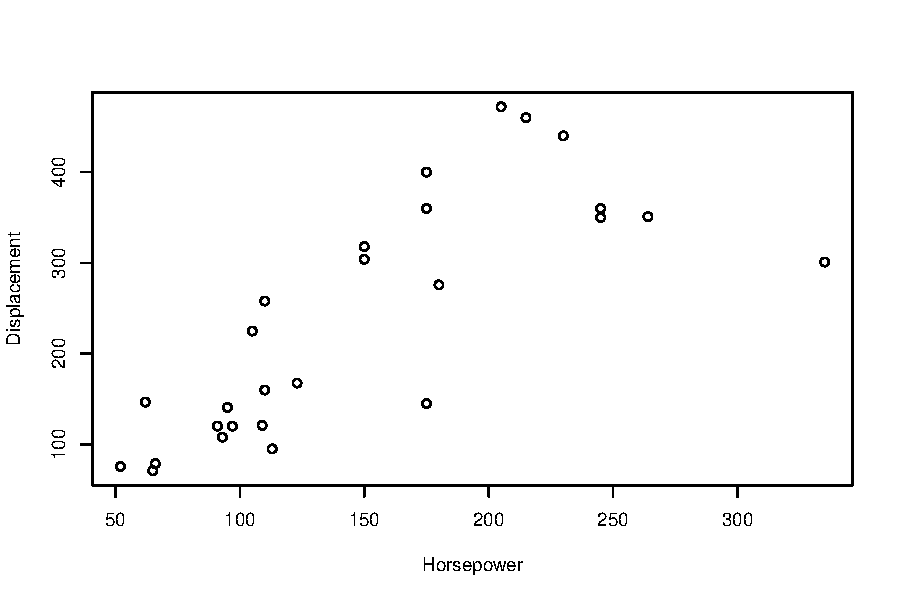
\includegraphics[width=\textwidth]{carfig.pdf}
  \caption{Here is a figure}
  \label{fig:cars}
\end{figure}

\section{Discussion}
\label{sec:disc}

Discussion about how the main points of the paper, limitations and future concerns.


\bibliography{refs.bib}
\bibliographystyle{plainnat}

\end{document}